%
% The first command in your LaTeX source must be the \documentclass command.
\documentclass[sigconf]{acmart}

%
% defining the \BibTeX command - from Oren Patashnik's original BibTeX documentation.
\def\BibTeX{{\rm B\kern-.05em{\sc i\kern-.025em b}\kern-.08emT\kern-.1667em\lower.7ex\hbox{E}\kern-.125emX}}
    

\copyrightyear{2018}
\acmYear{2018}
\setcopyright{acmlicensed}
\acmConference[Woodstock '18]{Woodstock '18: ACM Symposium on Neural Gaze Detection}{June 03--05, 2018}{Woodstock, NY}
\acmBooktitle{Woodstock '18: ACM Symposium on Neural Gaze Detection, June 03--05, 2018, Woodstock, NY}
\acmPrice{15.00}
\acmDOI{10.1145/1122445.1122456}
\acmISBN{978-1-4503-9999-9/18/06}

%
% These commands are for a JOURNAL article.
%\setcopyright{acmcopyright}
%\acmJournal{TOG}
%\acmYear{2018}\acmVolume{37}\acmNumber{4}\acmArticle{111}\acmMonth{8}
%\acmDOI{10.1145/1122445.1122456}

%
% Submission ID. 
% Use this when submitting an article to a sponsored event. You'll receive a unique submission ID from the organizers
% of the event, and this ID should be used as the parameter to this command.
%\acmSubmissionID{123-A56-BU3}

%
% The majority of ACM publications use numbered citations and references. If you are preparing content for an event
% sponsored by ACM SIGGRAPH, you must use the "author year" style of citations and references. Uncommenting
% the next command will enable that style.
%\citestyle{acmauthoryear}
\setcopyright{none}
\settopmatter{printacmref=false}
\renewcommand\footnotetextcopyrightpermission[1]{}
\pagestyle{plain}
%
% end of the preamble, start of the body of the document source.
\begin{document}

%
% The "title" command has an optional parameter, allowing the author to define a "short title" to be used in page headers.
\title{CSCI 622 Project Report: Phase-1}

%
% The "author" command and its associated commands are used to define the authors and their affiliations.
% Of note is the shared affiliation of the first two authors, and the "authornote" and "authornotemark" commands
% used to denote shared contribution to the research.
\author{Aravind Vicinthangal Prathivaathi}
\author {Griffin Dunn}
\author{Steven Simmons}
%
% The abstract is a short summary of the work to be presented in the article.
\begin{abstract}
The two most important cornerstone in any big data application is data security and privacy. Data security is a way of technically safeguarding the data from unauthorized use, while data privacy involved how this safeguarded data is being handled and the sensitivity of the individual attributes that make up the data. Our project's main focus is to explore new and interesting concepts involved in the security and privacy of our data and ultimately design an application that implements these concepts. We also intend to cover and analyze some prevalent issues surrounding the security and privacy of data. This phase-1 review of our project will be a quick introduction to our project, the data, it's schema and the software we use to store and access the data and the privacy and security concepts we intend to explore. 
\end{abstract}

%
% The code below is generated by the tool at http://dl.acm.org/ccs.cfm.
% Please copy and paste the code instead of the example below.
%
\begin{CCSXML}
<ccs2012>
 <concept>
  <concept_id>10010520.10010553.10010562</concept_id>
  <concept_desc>Computer systems organization~Embedded systems</concept_desc>
  <concept_significance>500</concept_significance>
 </concept>
 <concept>
  <concept_id>10010520.10010575.10010755</concept_id>
  <concept_desc>Computer systems organization~Redundancy</concept_desc>
  <concept_significance>300</concept_significance>
 </concept>
 <concept>
  <concept_id>10010520.10010553.10010554</concept_id>
  <concept_desc>Computer systems organization~Robotics</concept_desc>
  <concept_significance>100</concept_significance>
 </concept>
 <concept>
  <concept_id>10003033.10003083.10003095</concept_id>
  <concept_desc>Networks~Network reliability</concept_desc>
  <concept_significance>100</concept_significance>
 </concept>
</ccs2012>
\end{CCSXML}

% \ccsdesc[500]{Computer systems organization~Embedded systems}
% \ccsdesc[300]{Computer systems organization~Redundancy}
% \ccsdesc{Computer systems organization~Robotics}
% \ccsdesc[100]{Networks~Network reliability}

%%
%% Keywords. The author(s) should pick words that accurately describe
%% the work being presented. Separate the keywords with commas.
\keywords{datasets, anonymization, AWS, cloud, access control}

%% A "teaser" image appears between the author and affiliation
%% information and the body of the document, and typically spans the
%% page.
\begin{teaserfigure}
  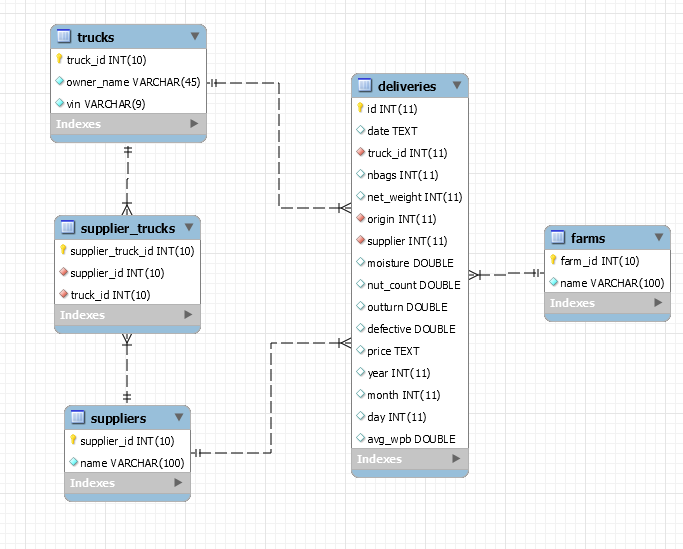
\includegraphics[width=\textwidth]{cashew_erd.png}
  \caption{Relational schema for Cashew Truck Arrivals}
  \Description{Relational schema for cashew truck arrivals dataset}
  \label{fig:teaser}
\end{teaserfigure}


\maketitle

\section{Introduction}

All organizations in this world have sensitive data that should be securely stored and have restricted access. With the world well into the digital age, the majority of the companies hold store data in clouds, privately owned servers and other distributed systems. Data protection, as a result, has become the top priority for any company. Breach of sensitive data could wreak havoc among a company's user-base, it's partners and it's employees.

Data security usually involves maintaining the integrity and accessibility of data. It ensures that data is accessed through secure channels and every user needs some authorization to view the data. This authorization may involve restrictions in manipulating, viewing, destroying or creating the data. On the other hand, data privacy is defined as the way data is handled. Policies must be created by each organization around how data is shared and used, this policy must then be open to the public and must be strictly followed by the company. Privacy policies usually differ with respect to the data that is being collected. Overall, we can say that the higher the sensitivity of data being collected and stored, the stronger should be the data security features and the respective policy. 

In our project, we intend to build a simple application interface or API which will allow us to query a database hosted on a server or cloud. Our plan is to build a system that initially doesn't have any privacy policies and lacks adequate security. We will then show that private data leaks can take place without appropriate data security, and we will show the importance of implementing these concepts mentioned earlier and how they will help secure the database from attacks and unauthorized users. Finally, we will implement the concepts mentioned earlier, show the difference between the initial insecure application and the final secure one. We shall also be exploring data security and privacy concepts such as database auditing, data access controls, application security, database hardening, some common attacks such as SQL injections and also investigate privacy policies in our project. We will look into the ethical issues surrounding data privacy as well. 


\section{Project Plan}
The below subsections will provide a brief overview of our project plan, albeit prone to minor updates and alterations in the future.

\subsection{Summary of our plan}
We plan on building a  web interface application or an Application Programmable Interface(API) to query our data. Here, users who can access the data through the interface and there will another group of users who can access the database directly as well as through the interface. Access and querying the database is restricted for all users except special ones. The database instance will be hosted on AWS. 

The initial application will have minimum security features, we will then analyze the different security threats and features applicable to our database [1,2,3,4,5,6,7], implement the relevant security features and do a comparative analysis between the initial application and the final one in terms of improvement in security. We shall then define privacy policies for our data.


\subsection{Data and it's schema}

We will be using a Cashew Truck Arrivals dataset which contains cashew nut deliveries to port houses from their respective farm over three years. The data is around 61 KB but we can create more data if a larger dataset is needed. 

The dataset contains 16 attributes and we use a relational database model to store and access the data. The schema for our relational database is shown in Figure 1. In the upcoming phase, we intend to implement integrity constraints and other security features over this schema. There is already a good potential number of sensitive data in our data set like owner\_name, origin\_farm and we plan to explore more. 

\subsection{Application and database}
We plan on building a relational web interface application or an Application Programmable Interface(API) to query our data. We intend to add security and privacy policies to our application as well on how it allows users to access data. Our application will make sure only authorized users can access data. 

We will be using Postgres as our data management system and a database instance hosted on AWS. Currently, our database is hosted on AWS at 54.210.93.153 where a postgres instance is running. We have created 3 separate users for each member of the team, each user is password protected and have complete permission to modify the database, as well as view, create and delete relations. 

\subsection{Security and privacy concepts}
Our project will have an application interface, a database, and a server where the database is hosted which could potentially lead to various data security threats. We shall research security threats involving lack of data audits, poor access control, data management, data leaks, SQL injections, and other application-level threats to data confidence and integrity[3,4,6,7]. 

We shall naturally also focus on the three pillars of data security: 1. Confidentiality, 2. Integrity and 3. Availability. We want to make sure that authorized users can always access data at any time through a secure channel. Hence, access control will be a major part of our system, each user will be a put in an access group with different permissions. For example, admins can create, manipulate, view or delete relations and data within the database, while regular users cannot only view data that they are authorized to but can neither delete existing data nor manipulate it. All data created by regular users must be through the interface. No regular user can be allowed to access the database directly. Different categories of users can always be added in the future with different permissions by the admins. 

We also want to explore different security concepts which include query restrictions, anonymization [5], cloud computing security issues[2], new access control techniques[1], authorization, and database auditing. 

\begin{enumerate}
    \item Query Restriction: There might be users other than admins, such as software engineers or testers who may want to access the database directly. Such users should have restrictions on the queries they can run. For example, in our dataset, they cannot execute queries to view the owner\_name but can always execute queries to view the number of owners.
    \item Anonymization: It is a way to de-identify data records stored in the cloud.  This could potentially reduce the burden on access control as it could encrypt sensitive data to users that do not have authorization.
    \item New access control techniques: Role-based access control and mandatory access control [1] are some methods we plan on exploring.
    \item Authorization: Every user except admins will have restricted access to data  and every user will be password protected.
    \item Database auditing: We plan on using software and logging systems to monitor our database, the different users who access it, what they access and potential problems related to security and privacy.
    
\end{enumerate}
We also plan on investigating existing tools and software that will help secure our database or alert us to potential threats to security policies or the lack of it.
We will also investigate the privacy issues regarding our data and the sensitive information we might need to restrict or hide from different users.

\begin{thebibliography}{9}

\bibitem{Data Security} 
    Elisa Bertino,
    \textit{ "Data mining with big data," in Data & Knowledge Engineering 25 (1998) 199-216}. 

\bibitem{Data Security and Privacy Protection Issues in Cloud Computing} 
 D. Chen and H. Zhao,
     \textit{ "Data Security and Privacy Protection Issues in Cloud Computing," 2012 International Conference on Computer Science and Electronics Engineering, Hangzhou, 2012, pp. 647-651.}
     
\bibitem{Security of Big Data: A Review} 
    R. Bhatia and M. Sood,
    \textit{"Security of Big Data: A Review," 2018 Fifth International Conference on Parallel, Distributed and Grid Computing (PDGC), Solan Himachal Pradesh, India, 2018, pp. 182-186.}
     
\bibitem{Security and privacy for big data: A systematic literature review} 
    B. Nelson and T. Olovsson,
     \textit{ "Security and privacy for big data: A systematic literature review," 2016 IEEE International Conference on Big Data (Big Data), Washington, DC, 2016, pp. 3693-3702.}. 
     
 \bibitem{Making Big Data, Privacy, and Anonymization Work Together in the Enterprise: Experiences and Issues} 
    Sedayao, Jeff & Bhardwaj, Rahul & Gorade, Nakul.
    \textit{ "Making Big Data, Privacy, and Anonymization Work Together in the Enterprise: Experiences and Issues," Proceedings - 2014 IEEE International Congress on Big Data, BigData Congress 2014. 10.1109/BigData.Congress.2014.92. }. 

\bibitem{Big Data - Security and Privacy} 
    E. Bertino,
    \textit{ "Big Data - Security and Privacy," 2015 IEEE International Congress on Big Data, New York, NY, 2015, pp. 757-761.}. 

\bibitem{Big data privacy: a technological perspective and review} 
    Jain, P., Gyanchandani, M. & Khare, N.
    \textit{Big data privacy: a technological perspective and review. J Big Data 3, 25 (2016). https://doi.org/10.1186/s40537-016-0059-y}



\end{thebibliography}

\end{document}
